\documentclass[conference]{IEEEtran}
\IEEEoverridecommandlockouts
% The preceding line is only needed to identify funding in the first footnote. If that is unneeded, please comment it out.
\usepackage{cite}
\usepackage{amsmath,amssymb,amsfonts}
\usepackage{algorithmic}
\usepackage{graphicx}
\usepackage{textcomp}
\usepackage{xcolor}


\begin{document}

\title{IELTS Writing Task 1\\}

\author{\IEEEauthorblockN{Liu Zhaohong}}

\maketitle

\section{Dynamic Graph}

\subsection{Line Graph(past time)}

\textbf{The graph below shows the quantities of goods transported in the UK between 1974 and 2002 by four different modes of transport.}

\textbf{Summarize the information by selecting and reporting the main features, and make comparisons where relevant.}

\begin{figure}[htbp]
    \centerline{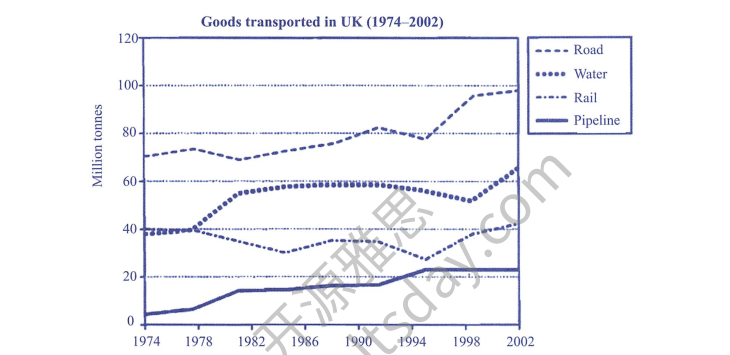
\includegraphics[width=1.4\columnwidth]{images/Screenshot from 2022-12-03 15-25-38.png}}
\end{figure}

The graph compares the volumes of goods delivered by four means of transport in the UK during the period 1974 to 2002.

The amount of goods transported by road was the largest, with around 70 million tonnes in 1974. 
It sharply increased to about 100 million tonnes in 2002. 
The figure for water was lower throughout the period: 
it rose from around 40 million tonnes in 1974 to about 58 million tonnes in 1980 and then stood at this level until 1998, 
before climbing to over 65 million tonnes in 2002.

The amounts of goods transported by the other two means of transport were lower. 
There was a dramatic fall in the figure for rail transportation from around 40 million tonnes on 1974 to 30 million tonnes in 1984, 
although it increased to over 40 million tonnes in 2022. 
The pipeline for transporting goods saw a steady growth from approximately 5 million tonnes in 1974 to over 20 million tonnes in 1995, 
and then it remained at this level in the rest of the period. Despite the growth, it was the least popular means of transport.

Overall, almost every means of transport in UK saw an upward trend in the goods delivery, 
while there was a different pattern in rail. Road transportation delivered more goods than any other means of transport.

\begin{itemize}
    \item compare
    \item transport=deliver, good
    \item by 4 means of transport
    \item during the period 1974 to 2002
    \item amount, figure, amount for goods, figure for water
\end{itemize}

\subsection{Line Graph(past to future)}

\textbf{The graph below gives information from a 2008 report about consumption of energy in the USA since 1980 with projections until 2030.}

\textbf{Summarise the information by selecting and reporting the · main features and make comparisons where relevant.}

\begin{figure}[htbp]
    \centerline{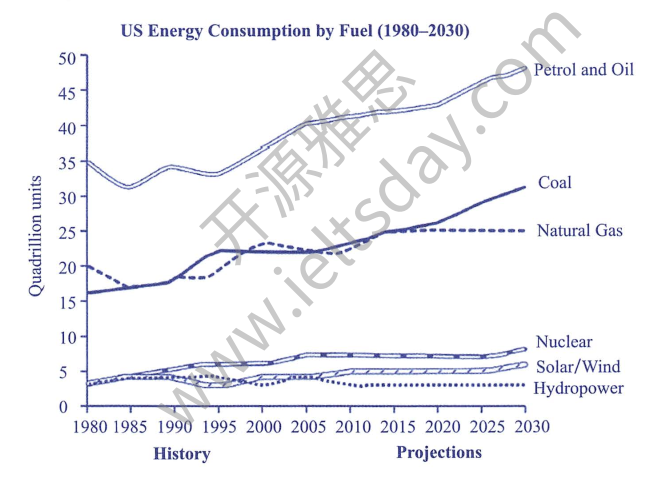
\includegraphics[width=1.0\columnwidth]{images/Screenshot from 2022-12-04 14-19-49.png}}
\end{figure}

The line graph shows the use of different sources of energy in the US over a 50-year period between 1980 and 2030.

Petrol and oil are the most important energy sources from 1980 to 2030. 
The consumption of these two fuels increased steadily and is expected to grow to 50 quadrillion units in 2030. 
There will be a similar trend in the consumption of coal, rising from around 17 q in 1980 to 30 q in 2030. 
It will become the second most important fuel. 
The consumption of natural gas saw a slight increase to about 25 q units in 2015 and will remain at this level in the rest of the period.

In contrast, the consumption of new energy sources, including nuclear, solar/wind and hydropower, is much lower. 
There will be a steady rise to nearly 9 quadrillion in nuclear consumption in 2030.  
The consumption of solar/wind will climb to over 5 quadrillion, while the figure for hydropower is predicted to fall to around 3 quadrillion.

Overall, fossil fuels will still be more important than environment-friendly alternative in the US. 
The energy production for all resources is expected to rise to various degrees, whereas the use of hydropower will show a different pattern.

\subsection{Pie Chart}

\textbf{Surveys conducted in 1982 and 2002 show different pictures of what motivate students to choose a college or university in the UK}

\textbf{Summarise the information by selecting and reporting the main features and make comparisons where relevant}

\begin{figure}[htbp]
    \centerline{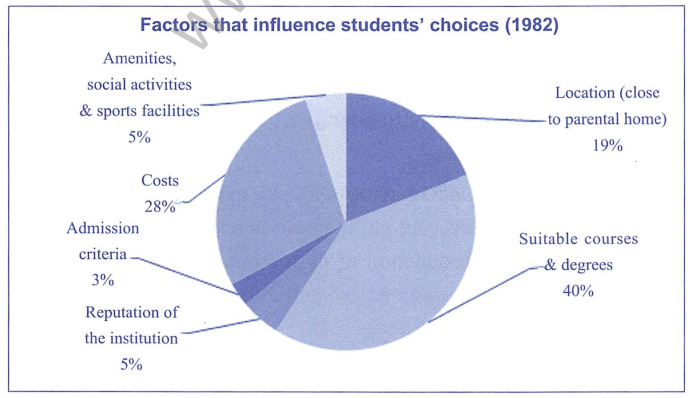
\includegraphics[width=1.0\columnwidth]{images/Screenshot from 2022-12-04 17-38-02.png}}
\end{figure}

\begin{figure}[htbp]
    \centerline{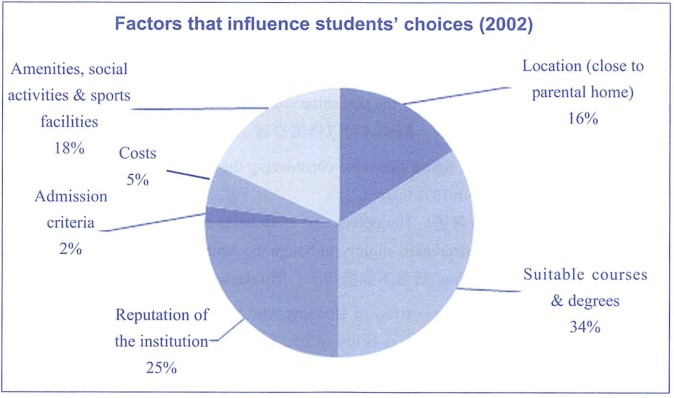
\includegraphics[width=1.0\columnwidth]{images/Screenshot from 2022-12-04 17-38-13.png}}
\end{figure}

The charts present the findings of a survey about what British students considered when choosing an university in two different years.

Pie charts compare the factors that students considered when choosing a university in the UK in two different years. 

suitable courses and degrees were the most popular consideration, although the proportion of students who cited this reason dropped from 40\% to 34\%. 
The percentage of students who considered costs was the second highest, but there was a sharp decrease to 5\%. 
Similar change happened to location factor either. The figure for those considering the distance to parental home declined from 19\% to 16\%.

In contrast, the proportion of students who paid attention to the reputation of the university was as low as 5\% in 1982, 
but this factor saw a significant rise to 25\%. 
There was a remarkable change in the percentage of people who valued amenities, social activities and sports facilities, rising from 5\% to 18\%. 
The figure for admission criteria remained basically unchanged(3\% in 1982 and 2\% in 2002).

Overall, more students considered suitable courses and degrees than those who focused on other factors. 
The percentages of students who considered fame of the university or amenities and sports facilities increased, 
while the figures for other factors showed opposing trends.

\subsection{Table}

\textbf{The table shows the amount of waste produced by different countries in 1980, 1990 and 2000}

\textbf{Summarise the information by selecting and reporting the main features, and make comparisons where relevant}

\begin{figure}[htbp]
    \centerline{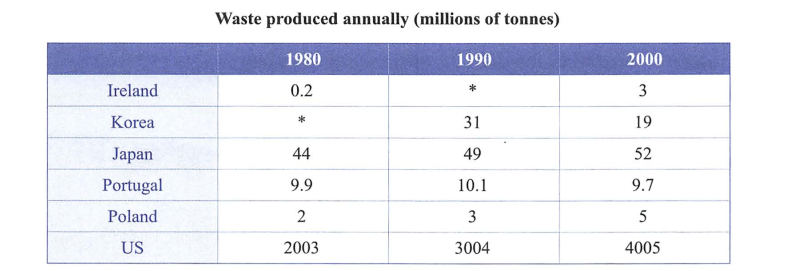
\includegraphics[width=1.1\columnwidth]{images/4.png}}
\end{figure}

The table provides information about the waste created in six countries in three separate years.

The waste produced by US was the highest, and it increased dramatically to 4005 million tonnes in 2000.
The figure for Japan was much lower, and there was a slight rise to 52 million tonnes.
Although no figure was given for Korea in 1980, the amount of waste produced by this country was huge(31 and 19 millions).

In contrast, the amounts of waste produced by other countries were much lower.
The figure for Ireland was the lowest, and there was no information for the year 1990.
Poland saw a slight increase from 2 million in 1980 to 5 million in 2000.
The figure for Portugal remained basically unchanged, climbing to 10.1 million and then decreasing to 9.7 million.

Overall, the US created more waste than any other country.
All countries created more waste during this period while Korea and Portugal saw different trends.

\subsection{Pie charts(Two objects to describe)}

\textbf{The pie charts below show units of electricity production by fuel source in Australia and France in 1980 and 2000.}

\textbf{Summarise the information by selecting and reporting the main features and make comparisons where relevant.}

\begin{figure}[htbp]
    \centerline{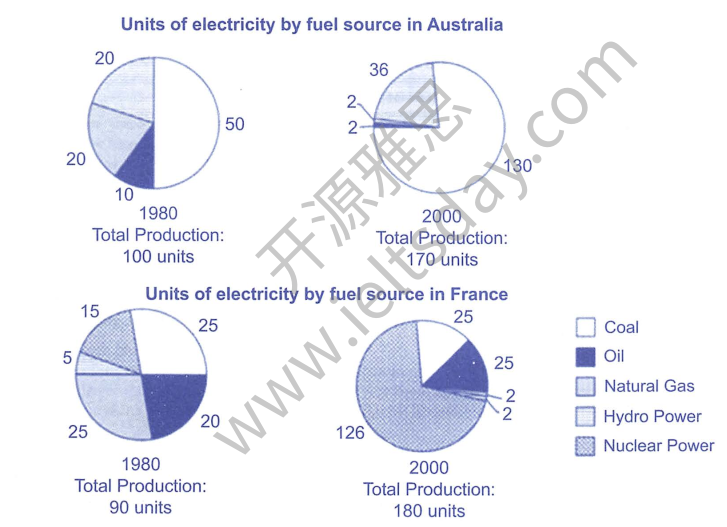
\includegraphics[width=1.1\columnwidth]{images/Screenshot from 2022-12-04 21-53-13.png}}
\end{figure}

The charts compare two countries in terms of the electricity produced by different fuels in 1980 and 2000.

The amount of electricity generated by coal was highest in Australia, and it increased from 50 to 130 units in 2000.
The figure for coal in France was much lower(25 units in both years).
There was a significant growth in the electricity created by nuclear power in France(from 15 units to 126 units).
The figure for hydro power increased from 20 to 36 units, although it was rather low in France(only 2 units in 2000).

Australia saw a drop in the electricity created by oil to 2 units in 2000, while France saw a rise to 25 units.
The figures for natural gas showed the same trend in these two countries, drooping to 2 units.

Overall, Australia relied more on coal than on any other energy source.
The amount of electricity generated by these two fuels increased in respective countries.

\subsection{Pie charts(Two objects to describe)}
\textbf{The charts below give information on the ages of the populations of Yemen and Italy
in 2000 and projections for 2050}

\textbf{Summarise the information by selecting and reporting the main features and make
comparisons where relevant.}

\begin{figure}[htbp]
    \centerline{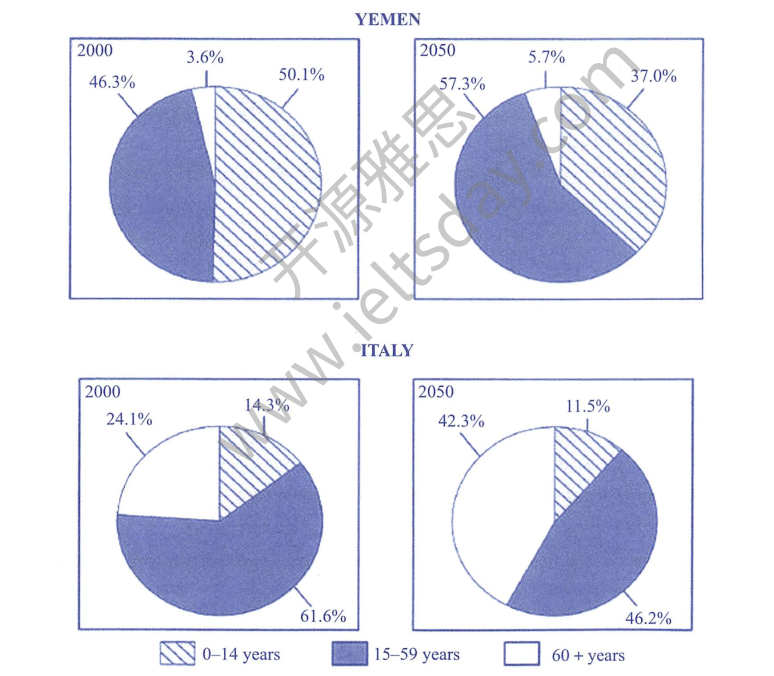
\includegraphics[width=1.1\columnwidth]{images/Screenshot from 2022-12-04 22-22-15.png}}
\end{figure}

The pie charts show the proportions of 3 different age groups in two countries in 2000, 
as well as projected figures for the year 2050.

In Yemen, people aged 15 to 59 are projected to represent the largest proportion of the population at 57.3\% in 2050,
up from 46.3\% in 2000.
A totally different pattern is expected to be seen in Italy for this age group,
with the figure dropping significantly from 61.6\% to 46.2\%,
although in both years, this age group was and will be the biggest one.

Both countries are likely to see an increase in the population aged 60 or older.
In Italy, the projection is that over-60s make up 42.3\% of the entire population, 
significantly higher than 24.1\% in 2000.
In Yemen, the growth is much smaller-from 3.6\% to 5.7\%.

As for the youngest group, these two countries may experience the same change.
The proportion of those aged 14 or younger in Yemen is likely to decline remarkably from 50.1\% to 37\%,
while only a modest decrease is predicted for Italy from 14.3\% to 11.5\%.

Overall, both countries are projected to see their population grow older in 2050, 
with a smaller proportion of those under the age of 14 and a larger proportion of those aged 60 or above.
In spite of these changes, the projection is that the 15-59 age group will be the biggest one in both countries.

\subsection{Bar Chart(Two objects to describe)}

\textbf{The charts give information about the proportions of boys and girls of a school who
achieved high grades (A or B +) in respective courses.}

\textbf{Summarise the information by selecting and reporting the main features, and make
comparisons where relevant.}

\begin{figure}[htbp]
    \centerline{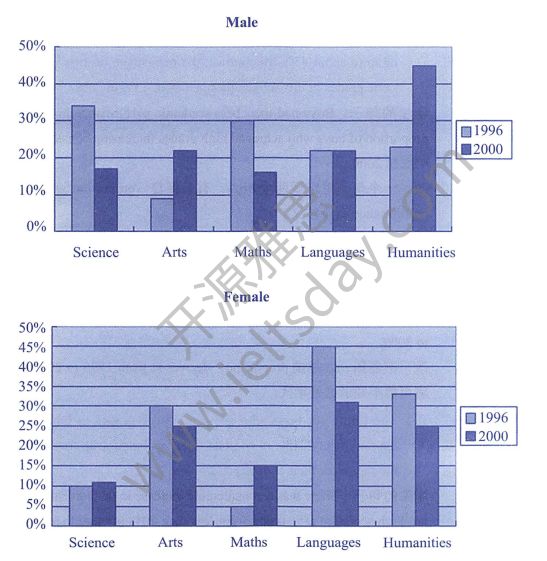
\includegraphics[width=1.1\columnwidth]{images/Screenshot from 2022-12-04 22-40-33.png}}
\end{figure}

The bar chart show the changes in the percentages of boys and girls gaining impressive grades in different subjects in 1996 and 2000.

Humanities saw the biggest increase in the proportion of high-achieving boys, with the figure nearly doubling to 43\% or so.
By comparison, the figure for girls drooped by 8\% to 25\%.
Similar changes happened to arts, in which the percentage of boys who gained high scores increased significantly to 21\% and
the figure for girls decreased slightly to 25\%.
Languages were another course which experienced a drop in the percentage of high-achieving girls, down to 31\%,
and the proportion of high-achievers for boys remained unchanged at about 21\% in this course.




\section{Static Graph}

\section{Flow Graph}

\section{Map Graph}


\end{document}